\chapter{Gesture recognition for Leap Motion}\label{GestureRecChapter}

\section{Classification of gestures}\label{classificationSection}

\begin{figure}[htb]
\centering
 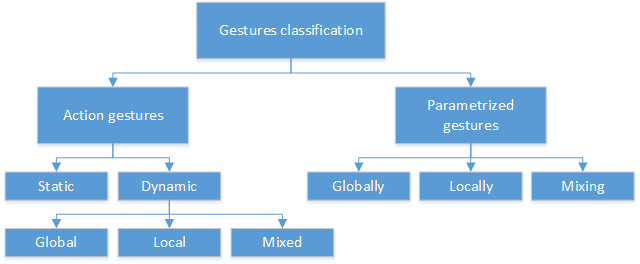
\includegraphics[width=0.8\columnwidth]{figures/gestureClassification.png}
 \caption[]{Classification of gestures proposed in the thesis}
 \label{thesisgesturetypes}
\end{figure}

In Section~\ref{taxonomySection} the three main classifications of gestures based on the existing literature have been presented. Particularly important for further research and to properly define the problem of gesture recognition may be the last of the presented taxonomies, which defines a wide range of possible gestures occurring in human-computer interaction.

It should be noticed that the previously mentioned classifications are defined strictly due to the characteristics of individual gestures, which may cause the selection of appropriate gesture recognition methods difficult. Therefore, it was decided to propose a new taxonomy that will be based on previously presented taxonomies~\cite{kammer_taxonomy_2010}\cite{Karam05ataxonomy}\cite{AignerTaxonomy} and in addition will be focused on the gesture recognition methods and will be defined strictly in the context of gesture recognition.

The proposed classification involves the following division by conveyed informations:
\begin{itemize}
\item action gestures (1),
\item parametrized gestures (2).
\end{itemize}

The former group (1), represents gestures, which their identification is based only on detection of gesture occurence. This means that action gestures have assigned some meaning, and the occurrence of this type of gesture implies execution of pre-defined action. It should also be noted that gestures of this type do not convey any additional parameters which define or describe the action. An example of this type can be gesture showing open hand, which could mean stop playing music. Another example might be a moving index finger in circles, which means rotating previously selected object of the specified number of degrees.

Gestures, which may be included into a parameterized gestures (2), provide additional parameters related to the context of the gesture. In contrast to previous group, parametrized gestures carry additional meaning or parameters needed to perform the gesture. An example of this kind of gestures might be a similar gesture to the previously mentioned instance of action gestures --- making circles through moving finger --- but in this case --- in addition to returned information about recognized gesture --- a value of angle, which should be used to rotate selected object, is also be conveyed.

Action gestures (1) is divided into static (1.1) and dynamic (1.2). The former group relates to gestures, that are not variable in time, therefore hand posture, its position and rotation are fixed during hand gesture performing. It should also be mentioned that these gestures should be independent of the orientation relative to the environment and the occurrence of this gesture is detected only on the basis of hand posture.

Dynamic action gestures (1.2) refer to the group of gestures which are constant and non-parametrized variable over time in terms of hand posture, position and rotation in space. This group is further divided into global, local and mixed. Global were detected based on a fixed hand posture and specified movement, which may relate both to changes in position and rotation. In the case of local, hand posture is only variable in time, while the mixed include gestures, for which both the hand posture, as well as the position and rotation vary with time. 

For parameterized gestures (2) division of locally (1.1), globally (1.2) and mixed parameterized gestures is distinguished. Globally parameterized gestures include gestures, whose parameters are determined by values of position and rotation or its changes of the hand. For instance, swipe gesture can be considered as globally parametrized gesture, where the parameter is the length of the swipe motion. Recognition of globally parametrized gestures is performed on the basis of unchanging hand posture or specific changes in the shape of the hand posture over time.

Locally parameterized gestures (1.2) include gestures whose the hand posture or its changes are parameterized, for example a distance between index finger and thumb of one hand may be a parameter for scaling gesture. Gestures of this kind should be independent of the position and rotation in space. Recognition should be based on the hand posture, which can be problematic when it will be time-varying.

Mixed parametrized group (1.3) represents gestures which both
\begin{itemize}
\item hand posture or hand posture changes over time,
\item and hand posture values or changes of position and rotation
\end{itemize}
are parametrized. Gestures of this group are recognized based on hand posture.
Classification presented above relates to the previously described taxonomy proposed by Aigner et al. at follows:
\begin{itemize}
\item pointing gestures -- represented by mixed parametrized gestures,
\item static semaphoric -- represented by static action gestures,
\item dynamic and stroke semaphoric -- represented by dynamic action gestures,
\item static iconic -- for demonstrating the shapes of objects represented by static action gestures and for presenting the size of object by locally parametrized gestures,
\item dynamic iconic -- mainly represented by dynamic action gestures, but can also be globally parameterized gestures for indicating the size of the objects,
\item pantomimic -- represented mostly by mixed dynamic action gestures, assuming that they are always performed in the same way,
\item manipulation -- represented by all types of parametrized gestures.
\end{itemize}

In this thesis all mentioned types of action gestures are considered. Recognition approaches of static action gestures are described in Chapter~\ref{staticChapter} and methods for dynamic action gestures are presented in Chapter~\ref{dynamicChapter}. Support for parametrized gestures by LeapGesture is envisaged for the further development of the library.

\section{Gesture data representation} \label{datarepSection}

LeapSDK provides built-in classes representing real--world object seen by the controller. The basic data unit we get from Leap Motion is a Frame. Frame contains objects like Hands and Pointables (Fingers and Tools), described by features directly related real attributes.

Hand is an object representing a regular human hand. It contains Fingers, and is described by three dimensional values, like: position of center of hand, normal vector and direction vector (pointing from the center to the end of fingers). 

Pointables are objects like Fingers or Tools (which are longer and thinner than Fingers). Both are described by the same set of features: position of tip, pointing direction vector, length and width.

\begin{itemize}
	\item Frame:
	\begin{itemize}
		\item Hands (position of center, normal vector, direction vector)
			\begin{itemize}
				\item Pointables: (tip position, pointing direction, length, width)
				\begin{itemize}
					\item Fingers
					\item Tools
				\end{itemize}
			\end{itemize}
	\end{itemize}
\end{itemize}

All positions are expressed in milimeters, relative to position of controller which is always located in the center of the 3D space. Manufacturer claims, that the accuracy of device is about 0.01mm. Experiments shown results better than 0.2mm, using an industrial robot moving an object in controllers' field of view. This is more than enough, as accuracy of positioning human hand is about 0.4mm.~\cite{lmAN} 

\section{Preprocessing} \label{PreprocessingSection}

Stability of images acquired by Leap Motion can vary, which results in captured noisy data -- sometimes fingers may flicker, or non-existing objects appear in a view. Those malfunctions happen for a very short period of time, usually less then 5 frames. 

To improve data stability, a simple preprocessing has been proposed. Its principle is based on a median filter -- it uses a window with custom defined size. For a given frame, for every unique finger which have been captured in the window, the algorithm checks if it should be present in a current frame, by checking its neighbour frames.
The neighbourhood of width $w$ is understood as $w/2$ frames that were recorded earlier that currently analyzed frame and $w/2$ frames that were recorded later. 
In this neighbourhood, the occurrences of a finger ($f_0$) are counter and decision is made:

\begin{itemize}
\item if $f_0 > w/2$ then a finger should appear in that frame,
\item otherwise, a finger is believed to be a noise in the data.
\end{itemize}

If the finger does not exist in a current frame and described check indicates that it should, then its position is calculated using linear interpolation of finger positions in two closest frames. Otherwise, a finger is simply removed.

It is worth noticing, that preprocessing introduces delay in data transmission to the next processing blocks of gesture recognition. 
Using wider width of preprocessing linearly causes greater delay.
For example, while capturing data with framerate equal to 50 frames per second and window size equal four, the delay would be:

$$ \frac{w/2+1}{fps} = \frac{3}{50} = 0.06s $$

The delay of $0.06s$ is not affecting the recognition speed, but larger windows may introduce noticeable delay. 
